\documentclass[sigconf,review, table]{acmart}

\usepackage{xcolor}
\usepackage{graphicx}
\usepackage{float}

\usepackage{booktabs}
\usepackage{multirow}

\setcopyright{acmcopyright}
\copyrightyear{2019}
\acmYear{2019}
\acmDOI{10.1145/1122445.1122456}
\acmMonth{8}

\acmConference[ICSE 2020]{Technical Papers}{May
23--29}{Seoul, North Korea}

\begin{document}

\title{Improving Software Maintainability through Automated Refactoring of Code Clones}

\author{Simon Baars}
\affiliation{\institution{University of Amsterdam}}
\email{simon.mailadres@gmail.com}

\author{Ana Oprescu}
\affiliation{\institution{University of Amsterdam}}
\email{ana.oprescu@uva.nl}

\begin{abstract}
Duplication in source code is often seen as one of the most harmful types of technical debt because it increases the size of the codebase and creates implicit dependencies between fragments of code. To remove such anti-patterns, the codebase should be refactored. Many tools aid in the detection process of such duplication problems, but failed to determine whether a duplicate fragment would improve the maintainability of the codebase when refactored.

We perform an exploratory study into the data that can be gathered from comparing before- and after snapshots of an automatically refactored system. We propose a tool to detect clones, analyze their context and automatically refactor a subset of them. We use a set of metrics to determine the impact of the applied refactorings to the maintainability of the system. On the basis of these results, we decide which clones improve system design and thus should be refactored. %We identified a set of four factors that influence the maintainability impact of clones. The first is the size of the clone. The second is the relation between the code fragments in a clone. The third is whether the clone fragments create, modify or return data. The fourth is the amount of data that cloned fragments use. By using these four factors, we can suggest only clones that will improve maintainability when refactored and prioritize them accordingly.
Given these maintainability influencing factors and their effect on the source code, we measure their impact over a large corpus of open source Java projects. %This results in a set of thresholds by which clones can be found that should be refactored to improve system maintainability.

We have identified that the size of the duplication problem is the biggest influencing factor on system maintainability. We found that the majority of duplicates spanning 29 or more tokens improve maintainability when refactored. Another maintainability influencing factor is the amount of data that needs to be passed to the merged location of the duplicate.
\end{abstract}

\keywords{code clones, refactoring, static code analysis, object-oriented programming}

\maketitle

\section{Introduction}
Duplicate fragments in source code (also named ``code clones'') are often seen as one of the most harmful types of technical debt \cite{fowler2018refactoring}. Duplicate fragments create implicit dependencies that make the code harder to maintain as the resolution of erroneous behaviour in one location may have to be applied to all the cloned code as well \cite{ostberg2014automatically}. Apart from that, code clones can contribute up to 25\% of the code size~\cite{bruntink2005use}.

Current code clone detection techniques base their thresholds and prioritization on a limited set of metrics. Often, clone detection techniques are limited to measuring the size of clones to determine whether they should be considered. Because of this, the output of clone detection tools is often of limited assistance to the developer in the refactoring process.

In this study, we define a technique to detect clones such that they can be refactored. We evaluate the context of clones to determine which refactoring techniques are required to refactor clones in a specific context. We propose a tool for the automated refactoring of a subset of the detected clones, by extracting a new method out of duplicated code.

We use automated refactoring to compare the maintainability of the before- and after snapshots of a codebase for each duplication problem that is refactored. This gives us insight into whether clones detected by certain thresholds should be refactored to improve the maintainability of the codebase. This allows for more accurate suggestion of code clones for refactoring and can provide assistance in the refactoring process.

\section{Background}
This study researches an intersection of code clone and refactoring research. In this background section, we will explain the required background knowledge for terms used throughout this study.

\subsection{Code clone terminology}
In this study we use two concepts used to argue about code clones \cite{roy2007survey}:
\\ \textbf{Clone instance}: A single cloned fragment.
\\ \textbf{Clone class}: A set of similar clone instances.

%\subsection{Code clone definitions} Optional -> may do this if it adds something to the story
%Quick overview of clone type definitions

\subsection{Refactoring techniques}
In this section, we describe refactoring techniques that are relevant to refactoring code clones.

\subsubsection{Extract Method}
The most used technique to refactor duplicate code is ``Extract Method'' \cite{fowler2018refactoring}, which can be applied on code inside the body of a method. Several studies have already concluded that most duplication in source code is found in the body of methods \cite{lozano2007evaluating, white2016deep, bergman2004ethnographic}. The ``Extract Method'' technique moves functionality in method bodies to a new method. To reduce duplication, we extract the contents of a single clone instance to a new method and replace all clone instances by a call to this method.

\subsubsection{Move Method}
Often, ``Extract Method'' alone is not enough to refactor clones. This is because the extracted method has to be moved to a location that is accessible by all clone instances. To do this, we apply the ``Move Method'' refactoring technique \cite{fowler2018refactoring}. In object-oriented programming languages, we often move methods up in the inheritance structure of classes, also called ``Pull Up Method'' \cite{fowler2018refactoring}.

\section{Defining refactorable clones}
% Instead of defining clone types, I just define how we can ensure that clones can be refactored. I do not plan to differentiate between T1R, T2R, and T3R here, because I think it makes the paper confusing.
% To be honest, I'm not even sure how relevant it is to name the literature clone types. Maybe not focus on their shortcomings, but just start from the core (source code) and define how we can get to refactorable clones.
In literature, several clone type definitions have been used to argue about duplication in source code \cite{roy2007survey}. In this section, we discuss how we can define clones such that they can be refactored without side effects on the source code.

\subsection{Ensuring Equality}\label{sec:t1r}
% Explain type 1, why it is not always refactorable, solution
Most modern clone detection tools detect clones by comparing the code textually together with the omission of certain tokens \cite{roy2009comparison, svajlenko2014evaluating}. Clones detected by such means may not always be suitable for refactoring, because textual comparison fails to take into account the context of certain symbols in the code. Information that gets lost in textual comparison is the referenced declaration for type, variable and method references. Equally named type, variable and method references may refer to different declarations with a different implementation. Such clones can be harder to refactor, if beneficial at all.

To detect clones that can be refactored, we propose to:
\begin{itemize}
  \item Compare variable references not only by their name but also by their type.
  \item Compare referenced types by their fully qualified identifier (FQI). The FQI of a type reference describes the full path to where it is declared.
  \item Compare method references by their fully qualified signature (FQS). The FQS of a method reference describes the full path to where it is declared, plus the FQI of each of its parameters.
\end{itemize}

% Do we want an example here?

\subsection{Allowing variability in a controlled set of expressions} \label{sec:t2r}
%Explain type 2, why it is not always refactorable, solution
Often, duplication fragments in source code do not match exactly \cite{kodhai2013method}. Often when developers duplicate fragments of code, they modify the duplicated block to fit its new location and purpose. To detect duplicate fragments with minor variance, we looked into in what expressions we can allow variability while still being refactorable.

We define the following expressions as refactorable when varied:
\begin{itemize}
  \item \textbf{Literals}: Only if all varying literals in a clone class have the same type.
  \item \textbf{Variables}: Only if all varying variables in a clone class have the same type.
  \item \textbf{Method references}: Only if the return value of referenced methods match (or are not used).
\end{itemize}
Often when allowing such variance, trade-offs come into play. For instance, variance in literals may require the introduction of a parameter to an extracted method if the ``Extract Method'' refactoring method is used, increasing the required effort to comprehend the code.

\subsection{Gapped clones} \label{sec:t3r}
%Explain type 3, why it is not always refactorable, solution
Sometimes, when fragments are duplicated, a statement is inserted or changed severely for the code to fit its new context \cite{roy2007survey}. When dealing with such a situation, there are several opportunities to refactor so-called ``gapped clones''. ``Gapped clones'' are two clone instances separated by a ``gap'' of non-cloned statement(s). We define the following methods to refactor such clones:
\begin{itemize}
  \item We wrap the difference in statements in a conditionally executed block, one path for each different (group of) statement(s).
  \item We use a lambda function to pass the difference in statements from each location of the clone.
\end{itemize}
Again, a trade-off is at play, as these solutions increase the complexity in favor of removing a clone.

\section{CloneRefactor}
% NEED TO EXPLAIN WHY DO CURRENT DETECTION TOOLS NOT SUFFICE
% The tool: Detect Clones, Map Context, Refactor.
To automate the process of refactoring clones, we propose a tool named CloneRefactor\footnote{The source code of CloneRefactor is available on GitHub: \url{https://github.com/SimonBaars/CloneRefactor}}. This tool goes through a 3-step process to refactor clones. This process is displayed in Fig.~\ref{fig:clonerefactorflow}.
\begin{figure}[H]
  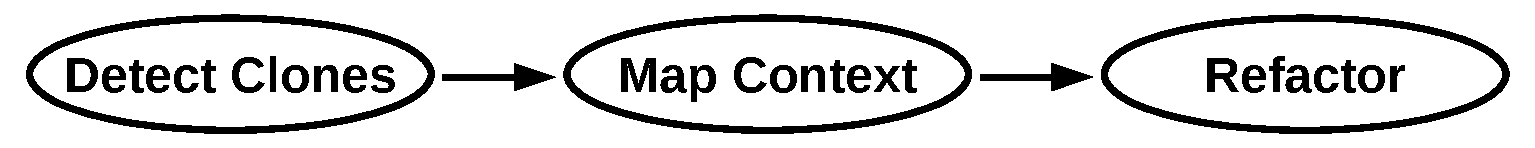
\includegraphics[width=1\columnwidth]{img/flow}
  \caption{Simple flow diagram of CloneRefactor.}
  \label{fig:clonerefactorflow}
\end{figure}
In this section, we explain each of these steps.

\subsection{Clone Detection}
% Detecting refactorable clones, (clone graph?? do I want to explain my exact methods?)
We use an AST-based method to detect clones. Clones are detected on a statement level: only full statements are considered as clones. In this process, we limit the variability between indicated expressions (see Sec.~\ref{sec:t2r}) by a threshold. This threshold is the percentage of different expressions against the total number of expressions in the source code:
\begin{equation}\label{eq:type2r}
\text{Variability}=\frac{\text{Different expressions}}{\text{Total expressions}}*100
\end{equation}

After all clones have been detected, CloneRefactor determines whether clone classes can be merged into gapped clones (see Sec.~\ref{sec:t3r}). The maximum size of the gap is limited by a threshold. This threshold is the percentage of (not-cloned) statements in the gap against the sum of statements in both clones surrounding it. Unlike the expression variability threshold, this threshold can exceed 100\%:
\begin{equation}\label{eq:type3r}
\text{Gap Size}=\frac{\text{Statements in gap}}{\text{Statements in clones}}*100
\end{equation}

To verify the correctness of all detected clones, we ran the tool over a large project and manually checked the output. We also created a set of control projects to test the correctness for many edge cases.

\subsection{Context Mapping} \label{sec:context}
After clones are detected, we map the context of these clones. We have identified three properties of clones as their context: relation and contents. We identify categories for each of these properties, to get a detailed insight into the context of clones.

\subsubsection{Relation}\label{sec:relation}
% The rationale for our categories regarding clone relations.
Clone instances in a clone class can have a relation with each other through inheritance. This relation has a big impact on how the clone should be refactored \cite{fontana2015duplicated}. We define the following categories to map the relation between clone instances in a clone class. These categories do not map external classes (classes outside the project, for instance, belonging to a library) unless explicitly stated:
\begin{itemize}
    \item \textbf{Common Class}: All clone instances are in the same class.
    \begin{itemize}
        \item \textbf{Same Method}: All clone instances are in the same method.
        \item \textbf{Same Class}: All clone instances are in the same class.
    \end{itemize}
    \item \textbf{Common Hierarchy}: All clone instances are in the same inheritance hierarchy.
    \begin{itemize}
        \item \textbf{Superclass}: Clone instances reside in a class or its parent class.
        \item \textbf{Sibling Class}: All clone instances reside in classes with the same parent class.
        \item \textbf{Ancestor Class}: All clone instances reside in a class, or any of its recursive parents.
        \item \textbf{First Cousin}: All clone instances reside in classes with the same grandparent class.
        \item \textbf{Same Hierarchy}: All clone instances are part of the same inheritance hierarchy.
    \end{itemize}
    \item \textbf{Common Interface}: All clone instances are in classes that have the same interface.
    \begin{itemize}
        \item \textbf{Same Direct Interface}: All clone instances are in a class that have the same interface.
        \item \textbf{Same Class}: All clone instances are in an inheritance hierarchy that contains the same interface.
    \end{itemize}
    \item \textbf{Unrelated}: All clone instances are in classes that have the same interface.
    \begin{itemize}
        \item \textbf{No Direct Superclass}: All clone instances are in classes that have the Object class as parent.
        \item \textbf{No Indirect Superclass}: All clone instances are in a hierarchy that contains a class that has the Object class as parent.
        \item \textbf{External Superclass}: All clone instances are in classes the same external class as parent.
        \item \textbf{Indirect External Ancestor}: All clone instances are in a hierarchy that contains a class that has an external class as parent.
    \end{itemize}
\end{itemize}

Based on these relations, we determine where to place the cloned code when refactored. The code of clones that have a \textit{Common Class} relation can be refactored by placing the cloned code in this same class. The code of clones with a \textit{Common Hierarchy} relation can be placed in the intersecting class in the hierarchy (the class all clone instances have in common as an ancestor). The code of clones with a \textit{Common Interface} relation can be placed in the intersecting interface, but in the process has to become part of the classes' public contract. The code of clones that are \textit{Unrelated} can be placed in a newly created place: either a utility class, a new superclass abstraction or an interface.

\subsubsection{Contents}\label{sec:contents}
% The rationale for our categories regarding clone contents.
The contents of a clone instance determine what refactoring techniques can be applied to refactor such clones. We define the following categories by which we analyze the contents of clones:
\begin{enumerate}
  \item \textbf{Full Method/Constructor/Class/Interface/Enumeration:} A clone that spans a full class, method, constructor, interface or enumeration, including its declaration.
  \item \textbf{Partial Method/Constructor:} A clone that spans (a part of) the body of a method/constructor.
  \item \textbf{Several Methods:} A clone that spans over two or more methods, either fully or partially, but does not span anything but methods.
  \item \textbf{Only Fields:} A clone that spans only global variables.
  \item \textbf{Other:} Anything that does not match with above-stated categories.
\end{enumerate}

\subsubsection{Full Method/Constructor/Class/Interface/Enumeration}
The categories denote that a full declaration (method, class, etc.) often denote redundancy and are often easy to refactor: one of both declarations is redundant and should be removed. Clones in the ``Partial Method/Constructor'' category can often be refactored using the ``Extract Method'' refactoring technique. Clones consisting of \textit{Several Methods} give a strong indication that cloned classes are missing some form of abstraction, or their abstraction is used inadequately. Clones consisting of \textit{Only Fields} often indicate data redundancy: different classes use the same data.

\subsection{Refactoring}
CloneRefactor can refactor clones using the ``Extract Method'' refactoring technique. In this section, we show which clones we refactor and how we apply these transformations.

\subsubsection{Extract Method}
% Show my categories to show what clones can be dealt with by method extraction.
Several influencing factors may obstruct the possibility to extract code to a new method:
\begin{itemize}
    \item \textbf{Complex Control Flow}: This clone contains \texttt{break}, \texttt{continue} or \texttt{return} statements, obstructing the possibility of method extraction.
    \item \textbf{Spans Part Of A Block}: This clone spans a part of a block statement.
    \item \textbf{Is Not A Partial Method}: If the clone does not fall in the ``Partial method'' category of Sec.~\ref{sec:contents}, the ``Extract Method'' refactoring technique cannot be applied.
    \item \textbf{Returns Multiple Values}: If a clone modifies or declares multiple pieces of data that it should return.
    \item \textbf{Top-Level Non-Statement}: If one of the top-level AST nodes of the clone is not a statement. For instance, if a (part of) an anonymous class is cloned.
    \item \textbf{Can Be Extracted}: This clone is a fragment of code that can directly be extracted to a new method. Then, based on the relation between the clone instances, further refactoring techniques can be used to refactor the extracted methods (for instance ``pull up method'' for clones in sibling classes).
\end{itemize}
Clones that do not fall in the \textit{Can Be Extracted} category may require additional transformations or other techniques to refactor. CloneRefactor only refactors the clones that \textit{Can Be Extracted}.

\subsubsection{AST Transformation}
% Explain what AST transformations I do to apply the refactorings.
CloneRefactor uses JavaParser \cite{tomassetti2017javaparser}: an AST-parsing library that allows to modify the AST and write it back to source code. To refactor clones, CloneRefactor creates a new method declaration and moves all statements from a clone instance in the clone class to the new method. This method is placed according to the relation between the clone instances (see Sec.~\ref{sec:relation}). CloneRefactor analyzes the source code of the extracted method and populates it with the following properties:
\begin{itemize}
  \item \textbf{Parameters}: For each variable used that is not accessible from the scope of the extracted method.
  \item \textbf{A return value}: If the method modifies or declares local data that is needed outside of its scope, or if the cloned fragments already returned data.
  \item \textbf{Thrown exception}: If the method throws an uncaught exception that is not a \texttt{RuntimeException}.
\end{itemize}
CloneRefactor then removes all cloned code and replaces it with a method call to the newly created method. In case of a return value, CloneRefactor either assigns the call result, declares it or returns it accordingly.

We verified the correctness of the resulting refactorings manually. We ran the tool over a large software project and verified over 1.000 applied refactorings.

\subsubsection{Characteristics of the extracted method}\label{sec:characteristics}
We define the following characteristics of the extracted method and/or the call:
\begin{itemize}
\item \textbf{Tokens}: The number of tokens in the body of the method.
\item \textbf{Relation}: The relation category (Sec.~\ref{sec:relation}) by which this methods' location was determined.
\item \textbf{Returns}: Whether the method calls return, declare, assign or don't use any data from the extracted method.
\item \textbf{Parameters}: The number of parameters the extracted method has.
\end{itemize}
We hypothesize that these characteristics are the main factors influencing the impact on the maintainability of the system as a result of refactoring the clone.

\subsubsection{Impact on maintainability metrics} \label{sec:metrics}
CloneRefactor measures the impact on maintainability metrics of the refactored source code for each clone class that is refactored. These metrics are derived from Heitlager et al. \cite{heitlager2007practical}. This paper defines a set of metrics to measure the maintainability of a system. For each of these metrics, risk profiles are proposed to determine the maintainability impact on the system of a whole.

To determine whether the maintainability improves when refactoring a single clone, we need to measure the impact of small-grained changes. Because of that, we measure only a subset of the metrics \cite{heitlager2007practical} and focus on the absolute metric changes (instead of the risk profiles). The subset of metrics we decided to focus on are all metrics that are measured on method level (as the other metrics show a lesser impact on the maintainability for these small changes). These metrics are:
\begin{itemize}
\item \textbf{Duplication}: In Heitlager et al. \cite{heitlager2007practical} this metric is measured by taking the amount of duplicated lines. We decided to use the amount of duplicated tokens part of a clone class instead, to have a stronger reflection of the impact of the refactoring by measuring a more fine-grained system property.
\item \textbf{Volume}: The more code a system has, the more code has to be maintained. The paper \cite{heitlager2007practical} measures volume as lines of code. As with duplication, we use the number of tokens instead.
\item \textbf{Complexity}: Heitlager et al. use MCCabe complexity \cite{mccabe1976complexity} to calculate their complexity metric. The MCCabe complexity is a quantitative measure of the number of linearly independent paths through a method.
\item \textbf{Method Interface Size}: The number of parameters that a method has. If a method has many parameters, the code may become harder to understand and it is an indication that data is not encapsulated adequately in objects \cite{fowler2018refactoring}.
\end{itemize}

\section{Experimental setup}
In this section, we describe the setup of our experiments.

\subsection{Corpus}
We ran all our experiments using CloneRefactor on a corpus of open source Java projects. This corpus is derived from the corpus of a study that uses machine learning to determine the suitability of Java projects on GitHub for data analysis purposes \cite{githubCorpus2013}.

CloneRefactor requires all libraries of the projects it analyses, to find the full paths of all referenced symbols in the source code (see Sec.~\ref{sec:t1r}). Because of that requirement, we decided to filter the corpus to only projects using the Maven build automation system. We created a set of scripts\footnote{All scripts to prepare the corpus are available on GitHub: \url{https://github.com/SimonBaars/GitHub-Java-Corpus-Scripts}} to prepare such a corpus with all dependencies included.

This procedure results in 2.267 Java projects including all their dependencies. The projects vary in size and quality. The total size of all projects is 14.2M lines (11.3M when excluding whitespace) over a total of 100K Java files. This is an average of 6.3K lines over 44 files per project. The largest project in the corpus is \textit{VisAD} with 502K lines.

\subsection{Minimum clone size}
In this study, we want to find out what thresholds to use to improve maintainability if clones by those thresholds are refactored. However, when clones are very small, they may never be able to improve maintainability. The detrimental effect of the added volume of the newly created method exceeds the positive effect of removing duplication. Because of that, we perform all our experiments with a minimum clone size of 10 tokens, because smaller clones cannot improve maintainability when refactored.

\subsection{Calculating a maintainability score}\label{sec:metricformula}
In this study, we use four metrics to determine maintainability \ref{sec:metrics}. For our experiments, we want to aggregate the scores obtained by these metrics to draw a conclusion about the maintainability increase or decrease after applying a refactoring. We base our aggregation on the following assumptions:
\begin{itemize}
  \item All metrics are equal in terms of weight towards system maintenance effort.
  \item Higher values for the metrics imply lower maintainability.
  \item The obtained increase of the metric divided by the average distance from zero over our corpus weights the metric equally against the other metrics.
\end{itemize}
We calculate the average deviation as follows:
\begin{equation}\label{eq:scoredev}
A = \frac{\sum_{x \in M} abs(x)}{|M|}
\end{equation}
Where \textit{M} is the multiset of all change in a certain metric for all refactorings over all systems in  obtained for a certain metric over our corpus and \textit{|M|} is the cardinality of this set. We then calculate the maintainability for a specific refactoring as follows:
\begin{equation}\label{eq:scoreref}
A_M = \frac{dup}{A_{dup}} + \frac{com}{A_{com}} + \frac{par}{A_{par}} + \frac{vol}{A_{vol}}
\end{equation}
Where \textit{dup} is the decrease in duplication, \textit{com} is the decrease in complexity, \textit{par} is the decrease is method parameters and \textit{vol} is the decrease in system volume after the refactoring is applied. When comparing the maintainability of a set of refactorings we divide the sum of the maintainability score by the amount of clone instances of all refactored clones in the set.

\section{Results}
In this section, we share the results of our experiments.

\subsection{Clone context}
% How many clones are there in certain contexts? Experiments for relation, location, and context.
To determine the refactoring method(s) that can be used to refactor most clones, we perform statistical analysis on the clone context (see Sec.~\ref{sec:context}).

\subsubsection{Relation}
Table~\ref{tab:relation} displays the number of clone classes found for the entire corpus for different relations (see Sec.~\ref{sec:relation}).

\begin{table}[H]
\centering
\begin{tabular}{@{}llll@{}}
\toprule
\textit{\textbf{Category}} & \textit{\textbf{Relation}} & \textit{\textbf{Clone Classes}} & \textit{\textbf{Total}} \\ \midrule
\multirow{2}{*}{\begin{tabular}[c]{@{}l@{}}Common\\ Class\end{tabular}} & Same Class & 22,893 & \multirow{2}{*}{31,848} \\ \cmidrule(lr){2-3}
 & Same Method & 8,955 &  \\ \midrule
\multirow{5}{*}{\begin{tabular}[c]{@{}l@{}}Common\\ Hierarchy\end{tabular}} & Sibling & 15,588 & \multirow{5}{*}{20,342} \\ \cmidrule(lr){2-3}
 & Superclass & 2,616 &  \\ \cmidrule(lr){2-3}
 & First Cousin & 1,219 &  \\ \cmidrule(lr){2-3}
 & Common Hierarchy & 720 &  \\ \cmidrule(lr){2-3}
 & Ancestor & 199 &  \\ \midrule
\multirow{4}{*}{Unrelated} & No Direct Superclass & 10,677 & \multirow{4}{*}{20,314} \\ \cmidrule(lr){2-3}
 & External Superclass & 4,525 &  \\ \cmidrule(lr){2-3}
 & External Ancestor & 3,347 &  \\ \cmidrule(lr){2-3}
 & No Indirect Superclass & 1,765 &  \\ \midrule
\multirow{2}{*}{\begin{tabular}[c]{@{}l@{}}Common\\ Interface\end{tabular}} & Same Direct Interface & 7,522 & \multirow{2}{*}{13,074} \\ \cmidrule(lr){2-3}
 & Same Indirect Interface & 5,552 &  \\ \bottomrule
\end{tabular}
\caption{Number of clone classes per clone relation}
\label{tab:relation}
\end{table}

\subsubsection{Contents}
Table~\ref{tab:contents} displays the number of clone classes found for the entire corpus for different contents (see Sec.~\ref{sec:contents}).

\begin{table}[H]
\centering
\begin{tabular}{@{}llll@{}}
\toprule
\textit{\textbf{Category}} & \textit{\textbf{Contents}} & \textit{\textbf{Clone instances}} & \textit{\textbf{Total}} \\ \midrule
\multirow{2}{*}{Partial} & Partial Method & 219,540 & \multirow{2}{*}{229,521} \\ \cmidrule(lr){2-3}
 & Partial Constructor & 9,981 &  \\ \midrule
\multirow{5}{*}{Full} & Full Method & 12,990 & \multirow{5}{*}{13,173} \\ \cmidrule(lr){2-3}
 & Full Interface & 64 &  \\ \cmidrule(lr){2-3}
 & Full Constructor & 58 &  \\ \cmidrule(lr){2-3}
 & Full Class & 37 &  \\ \cmidrule(lr){2-3}
 & Full Enum & 24 &  \\ \midrule
\multirow{3}{*}{Other} & Several Methods & 22,749 & \multirow{3}{*}{53,773} \\ \cmidrule(lr){2-3}
 & Only Fields & 17,700 &  \\ \cmidrule(lr){2-3}
 & Other & 13,324 &  \\ \bottomrule
\end{tabular}
\caption{Number of clone instances for clone contents categories}
\label{tab:contents}
\end{table}

\subsection{Extract Method}
%To what extent can found clones be refactored through method extraction, without requiring additional transformations.
Table~\ref{tab:refactorability} shows to what extent clone classes can be refactored by using the ``Extract Method'' refactoring technique. The second column shows our measurements for the complete systems (just like the former experiments). The third column shows our measurements when restricting our search to method bodies. The amount that can be extracted increases because, when restricting our search to method bodies, we do not exclude declarations that can obstruct the possibility of method extraction (for instance a cloned method signature).

\begin{table}[H]
\centering
\begin{tabular}{@{}lll@{}}
\toprule
\textit{\textbf{Category}} & \textit{\textbf{All}} & \textit{\textbf{Method Body}} \\ \midrule
Can Be Extracted & 24,157 & 26,109 \\
Is Not A Partial Method & 21,625 & 0 \\
Top-level AST-Node is not a Statement & 19,887 & 4,607 \\
Spans Part of a Block & 12,964 & 13,460 \\
Multiple Return Values & 5,622 & 6,131 \\
Complex Control Flow & 1,106 & 1,216 \\ \bottomrule
\end{tabular}
\caption{Number of clones that can be extracted using the ``Extract Method'' refactoring technique}
\label{tab:refactorability}
\end{table}

\subsection{Refactoring}
%I think the ultimate goal with this thesis is to do experiments with different clone thresholds. Which thresholds give clones that we should refactor? For this, we will measure the maintainability of the refactored source code over different thresholds. These thresholds range from minimum clone size, variability, and gap size.
In our corpus, CloneRefactor has refactored 12.710 clone classes and measured the change in indicated metrics (see Sec.~\ref{sec:metrics}). Using the presented formulas (see Sec.~\ref{sec:metricformula}) we determine how the characteristics of the extracted method (see Sec.~\ref{sec:characteristics}) influence the maintainability of the resulting codebase after refactoring. In this section, we explore the data received by comparing the before- and after snapshots of the system for each separate refactoring.

\subsubsection{Clone Token Volume}
Figure \ref{fig:duplication} shows the obtained results when plotting the clone size (in tokens) vs the maintainability increase/decrease. On the secondary axis the amount of refactorings that have refactored a clone with the specified amount of tokens is displayed (e.g. the amount of data points the data is based on). As the amount of data points decreases, the datapoints gain less statistical significance.

\begin{figure*}
  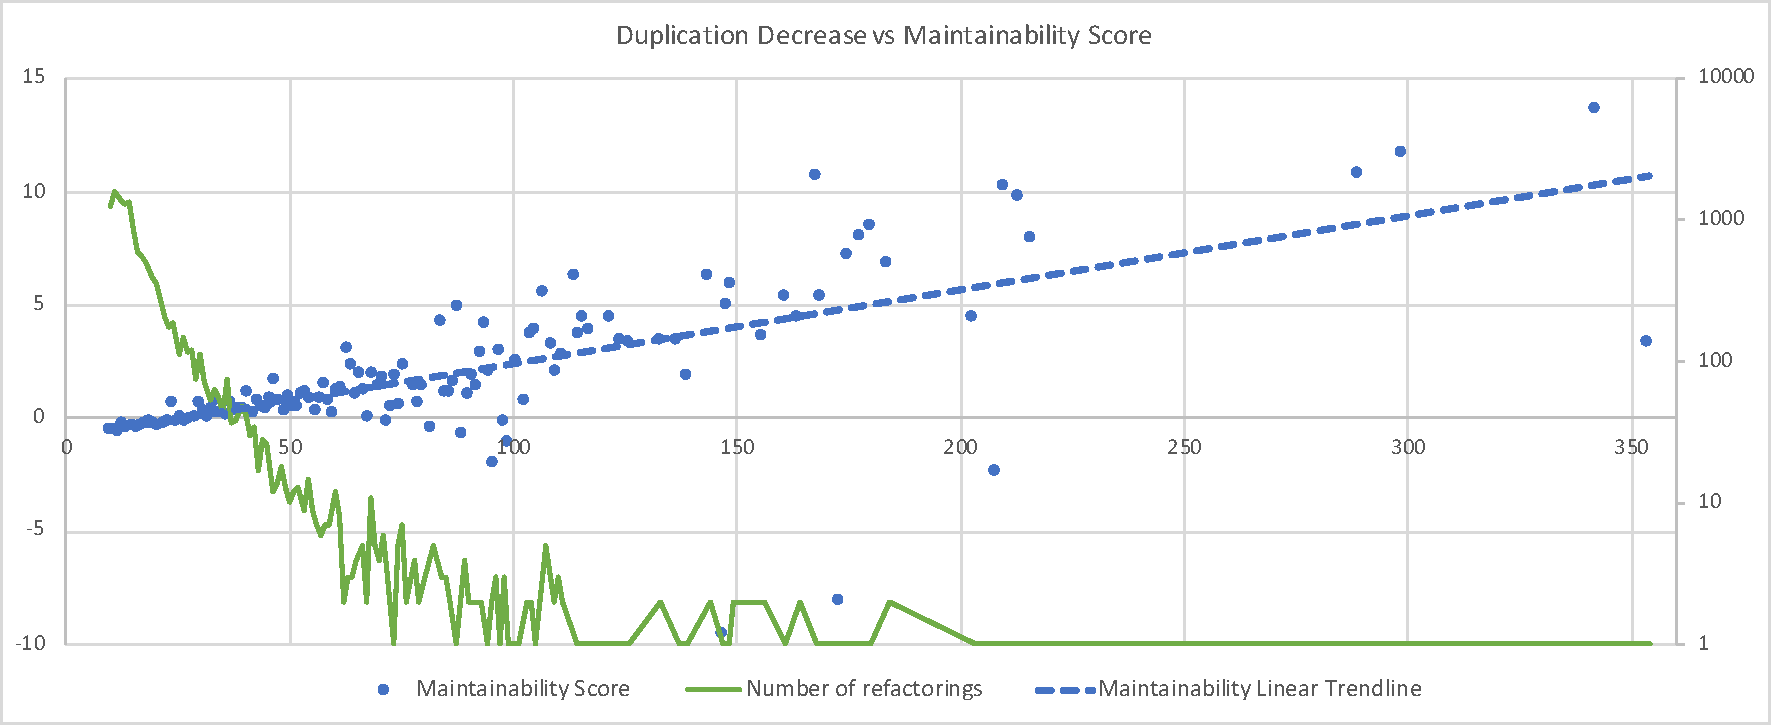
\includegraphics[width=1\textwidth]{img/duplication}
  \caption{A graph that shows how the size in tokens of the refactored clone affects maintainability. Maintainability on the primary axis and amount of refactorings on the secondary axis.}
  \label{fig:duplication}
\end{figure*}

The volume of the clone is the dominating factor regarding the maintainability increase/decrease of cloned code. Because of that, for our further experiments, we filter out all refactorings with a token size smaller than 18 because otherwise the small clones dominate the results and turn all results towards unmaintainable.

\subsubsection{Relation}
Table~\ref{tab:relation_refactor} shows our data regarding how different relations influence maintainability. We have marked rows based on less than 100 refactorings red, as their result does not have statistical significance.

\begin{table}[]
\centering
\begin{tabular}{@{}lll@{}}
\toprule
\textit{\textbf{Relation}} & \textit{\textbf{\begin{tabular}[c]{@{}l@{}}Maintainability\\ Score\end{tabular}}} & \textit{\textbf{\begin{tabular}[c]{@{}l@{}}Number of\\ Refactorings\end{tabular}}} \\ \midrule
\textbf{Common Hierarchy} & \textbf{0.51} & \textbf{792} \\ \midrule
\hspace{10pt} Sibling & 0.57 & 637 \\
\rowcolor[HTML]{FFCCC9}
\hspace{10pt} Same Hierarchy & 0.55 & 22 \\
\rowcolor[HTML]{FFCCC9}
\hspace{10pt} Superclass & 0.20 & 74 \\
\rowcolor[HTML]{FFCCC9}
\hspace{10pt} First Cousin & -0.02 & 53 \\
\rowcolor[HTML]{FFCCC9}
\hspace{10pt} Ancestor & -0.65 & 6 \\ \midrule
\textbf{Common Class} & \textbf{0.01} & \textbf{2,025}\\ \midrule
\hspace{10pt} Same Method & 0.01 & 762  \\
\hspace{10pt} Same Class & 0.01 & 1,263 \\ \midrule
\textbf{Unrelated} & \textbf{-0.02} & \textbf{688}\\ \midrule
\hspace{10pt} No Direct Superclass & 0.08 & 289 \\
\hspace{10pt} External Superclass & -0.02 & 225  \\
\rowcolor[HTML]{FFCCC9}
\hspace{10pt} No Indirect Superclass & -0.04 & 30  \\
\hspace{10pt} External Ancestor & -0.26 & 144  \\ \midrule
\textbf{Common Interface} & \textbf{-0.11} & \textbf{283} \\ \midrule
\hspace{10pt} Same Direct Interface & 0.02 & 160 \\
\hspace{10pt} Same Indirect Interface & -0.31 & 123
\end{tabular}
\caption{Influence on maintainability of refactoring clones by certain relations.}
\label{tab:relation_refactor}
\end{table}

\subsubsection{Return Value}
Table~\ref{tab:return} shows how the return value of the extracted method influences the maintainability of the resulting system.

\begin{table}[H]
\centering
\begin{tabular}{@{}lll@{}}
\toprule
\textit{\textbf{Return Value}} & \begin{tabular}[c]{@{}l@{}}\textit{\textbf{Maintainability}}\\\textit{\textbf{Score}}\end{tabular} & \begin{tabular}[c]{@{}l@{}}\textit{\textbf{Number of}}\\\textit{\textbf{Refactorings}}\end{tabular} \\ \midrule
Return & 0.20 & 421 \\
Void & 0.19 & 2052 \\
Declare & 0.03 & 1318 \\
\rowcolor[HTML]{FFCCC9}
Assign & -1.29 & 3 \\ \bottomrule
\end{tabular}
\caption{Maintainability scores for different return values}
\label{tab:return}
\end{table}

\subsubsection{Parameters}
Fig.~\ref{fig:arguments} shows how an increase in parameters lowers the maintainability of the refactored code. On the primary x-axis, the maintainability is displayed. The secondary x-axis shows the number of refactorings. The y-axis shows the number of parameters.

\begin{figure}[H]
  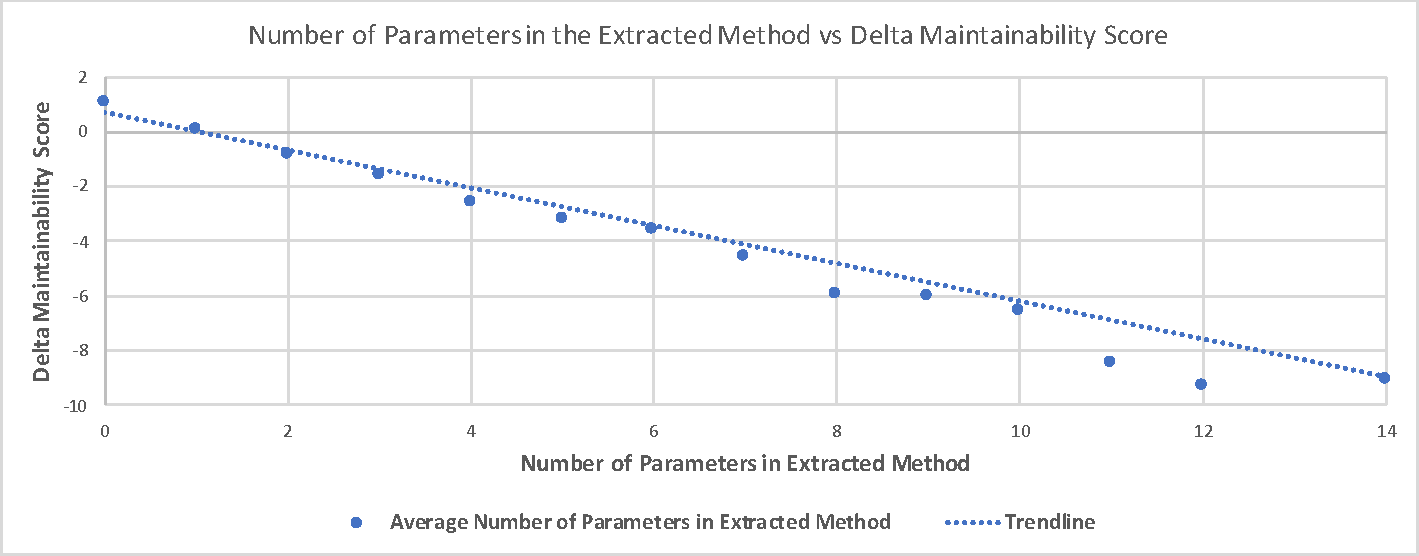
\includegraphics[width=1\columnwidth]{img/arguments}
  \caption{Influence of number of method parameters on system maintainability.}
  \label{fig:arguments}
\end{figure}

\section{Discussion}
In this section, we discuss the results of our experiments.

\subsection{Clone Context}
Regarding clone context, our results indicate that most clones (37\%) are in a common class. This is favorable for refactoring because the extracted method does not have to be moved after extraction. 24\% of clones are in a common hierarchy. These refactorings are also often favorable. Another 24\% of clones are unrelated, which is often unfavorable because it often requires a more comprehensive refactoring. 15\% of clones are in an interface.

Regarding clone contents, 74\% of clones span part of a method body (77\% if we include constructors). 8\% of clones span several methods, which often require refactorings on a more architectural level. 6\% of clones span only global variables, requiring an abstraction to encapsulate these data declarations. Only 4\% of clones span a full declaration (method, class, constructor, etc.).

\subsection{Extract Method}
28\% of clones can be refactored using the ``Extract Method'' refactoring technique (50\% if we limit our searching scope to method bodies). About 25\% of clones do not span part of a method, because of which they cannot be refactored. Many clones (23\%) do not have a statement as top-level AST-Node. Upon manual inspection, we noticed that the main reason for this is clones in anonymous functions or anonymous classes. About 15\% of clones span only part of an AST-Node.

\subsection{Refactoring}
In Fig.~\ref{fig:duplication} we see an increase in maintainability for refactoring larger clone classes. The tipping point, between a better maintainable refactoring and a worse maintainable refactoring, seems to lie around 28 tokens. There are fewer large clones than small clones, resulting in a very limited statistical significance on our corpus when considering clones larger than 100 tokens.

In Table~\ref{tab:relation_refactor} we see the results regarding refactorings that are applied to clones with diverse relations. We see that most refactored clones are in a common class, over 54\%. This is significantly more than the percentage of clones in the common class relation as reported in Table~\ref{tab:relation}. Meanwhile, the number of refactored unrelated clones is smaller than the number reported in Table~\ref{tab:relation} (24\% -> 18\%). The main reason for this is that refactoring unrelated clones can change the relation of other clones in the same system. If we create a superclass abstraction to refactor an unrelated clone, other clones in those classes that were previously unrelated might become related.

The maintainability scores displayed in Table~\ref{tab:relation_refactor} show that the most favorable clones to refactor are clones with a Sibling relation. The most unfavorable is to refactor clones to interfaces. However, the differences in maintainability in this table are generally small; there is no indication that relations have a major impact on the maintainability of clones.

Regarding the return type of refactored clones, we see in Table~\ref{tab:return} that this has no major impact on maintainability. A method call to the extracted method that is directly returned and no return type extracted methods are slightly more favorable than the others. We think the main reason that the ``Return'' category is on top is that when a variable is declared at the end of the cloned fragment, CloneRefactor directly returns its value and removes the declaration. This decreases the volume slightly.

A higher number of parameters directly influences the corresponding metric. Because of this, we see in Fig.~\ref{fig:arguments} that more parameters negatively influence maintainability. Not only the number of parameters metric is negatively influenced, but more method parameters also increase volume for the extracted method and each of the calls to it. Because of that, we see that trend of the graph in Fig.~\ref{fig:arguments} decreases relatively rapidly.

\section{Conclusion}
We defined refactorable clones and created a tool to detect and refactor them. We measured statistical data with this tool over a large corpus of open-source Java software systems to get more information about the context of clones and how refactoring them influences system maintainability.

We defined two aspects as part of the context of a clone: relation and contents. Regarding relations, we found that most clones are found in the same class, over 37\%. About 24\% of clones are in the same inheritance hierarchy. Another 24\% of clones are unrelated. The final 7\% of clones have the same interface. Regarding contents, over 74\% of clones span part of a method. About 8\% span several methods. Only 4\% of clones span a declaration (method, class, etc.) fully.

We built a tool that can automatically apply refactorings to 28\% of clones in our corpus using the ``Extract Method'' refactoring technique. The main reason our tool could not refactor all clones is that many clones span certain statements that obstruct method extraction, for instance when code outside a method is part of a clone.

We measured four maintainability metrics before- and after applying each refactoring to determine the impact of each refactoring on system maintainability. We found that the most prominent factor influencing maintainability is the size of the clone. We found that the threshold lies at a clone volume of 29 tokens per clone instance for system maintainability to increase after refactoring the clone. Another factor with a major impact on maintainability is the number of parameters that the extracted method requires to get all required data. We noticed that the inheritance relation of the clone and the return value of the extracted method has only a minor impact on system maintainability.

\section*{Acknowledgments}
We would like to thank the Software Improvement Group for their continuous support in this project. In particular, we would like to thank Xander Schrijen for his invaluable input in this research. Furthermore, we would like to thank Sander Meester for his proofreading efforts and feedback.

\bibliographystyle{ACM-Reference-Format}
\bibliography{references}

\end{document}
